\section{Progettazione}
Lo sviluppo del progetto si è basato sul pattern \textbf{Model-View} di \textit{Qt} e una metodologia mista \textit{top-down} e \textit{bottom-up}: si è infatti partiti con la metodologia \textit{top-down} per la progettazione della gerarchia e del container, ma durante la scrittura di \textit{model} e \textit{view} si è ripensato leggermente alla struttura di questi. \\
Oltre alla gerarchia, è stato realizzato un container templatizzato per il contenimento degli oggetti appartenenti alla gerarchia.
Sono stati realizzati inoltre:
\begin{itemize}
  \item Una \textit{GUI (Graphical User Interface)}, basata su classi preesistenti di \textit{Qt};
  \item Un \textit{model}, il quale si occupa della gestione dei dati del programma, basato anch'esso su classi preesistenti di \textit{Qt};
  \item Un \textit{filter proxy}, che funge da intermediario tra \textit{model} e \textit{view} e permette di filtrare i dati per la visualizzazione corretta su ogni tab;
  \item Una classe di Input/Output su file in formato \texttt{.xml}.
\end{itemize}

\begin{figure}[H]
  \centering
  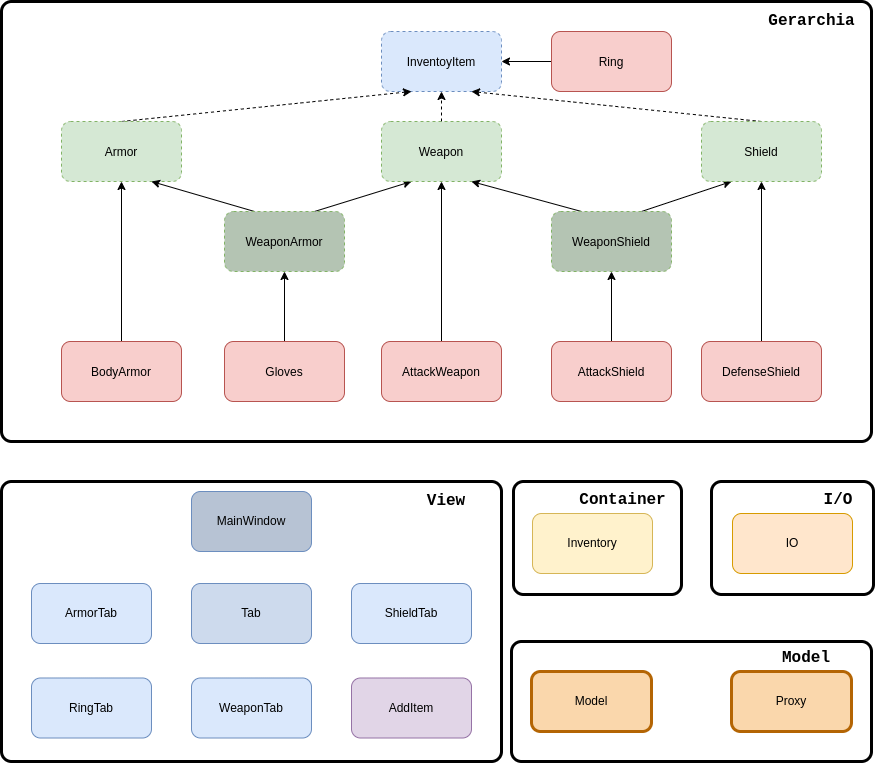
\includegraphics[width = \linewidth]{img/diagramma}
  \caption{Diagramma delle classi di CrownSouls.}
\end{figure}

\subsection{Gerarchia}
La gerarchia è composta dalla classe base astratta \textit{InventoryItem}, dalla quale derivano \textbf{direttamente} la classe concreta \textit{Ring} e \textbf{virtualmente} le classi astratte \textit{Armor}, \textit{Weapon} e \textit{Shield}. Da queste tre classi derivano \textbf{singolarmente} e \textbf{direttamente} le tre rispettive classi concrete \textit{BodyArmor}, \textit{AttackWeapon} e \textit{DefenseShield}. Viene inoltre utilizzata l'ereditarietà multipla per la definizione di classi che rappresentano oggetti appartenenti a più tipi; nello specifico, la classe \textit{WeaponArmor} deriva direttamente da \textit{Armor} e \textit{Weapon}, e la classe \textit{WeaponShield} deriva direttamente da \textit{Weapon} e \textit{Shield}. Questa forma di ereditarietà multipla è di tipo \textbf{is-a}, poiché un oggetto WeaponArmor è sia un oggetto Weapon che un oggetto Armor (e lo stesso vale per WeaponShield). Da queste due classi astratte derivano poi rispettivamente le classi concrete \textit{Gloves} e \textit{AttackShield}. \\
Ciascuna classe implementa dei metodi virtuali che riguardano l'impostazione e il recupero delle diverse proprietà degli elementi, e dei metodi virtuali specifici di ogni sottoclasse astratta per il calcolo e l'ottenimento di statistiche basate sulle proprietà. L'utilizzo del polimorfismo in tale contesto viene illustrato in seguito.

\subsection{Container}
È stata implementata una classe \textit{Inventory} che funge da container. La classe fornisce un template di smart pointer, e simula una lista singolarmente linkata con alcuni accorgimenti: a differenza di una lista singolarmente linkata standard, infatti, essa fornisce anche un puntatore all'ultimo elemento e permette l'accesso diretto in sola lettura a un dato elemento tramite l'overloading dell'operatore accesso agli elementi del puntatore (\textbf{[ ]}). \\
La classe \textit{Inventory} contiene al suo interno due classi annidate:
\begin{itemize}
  \item La classe \textit{SmartP} rappresenta uno smart pointer; è infatti questa classe a rappresentare un elemento del container di tipo T templatizzato. Oltre al contenuto effettivo dell'elemento e al puntatore all'elemento successivo, la classe è fornita anche di:
  \begin{itemize}
    \item Costruttore e costruttore di copia profondi;
    \item Distruttore profondo;
    \item Assegnazione profonda;
    \item Overloading degli operatori di dereferenziazione e accesso a membro;
    \item Overloading degli operatori booleani di uguaglianza e disuguaglianza.
  \end{itemize}
  \item La classe \textit{Iterator} rappresenta l'iteratore del container. Nello specifico, un oggetto di classe Iterator è un iteratore costante, poiché non permette il \textit{side effect} sugli oggetti a cui punta. Questa classe presenta l'overloading dei seguenti operatori:
  \begin{itemize}
    \item Incremento prefisso;
    \item Dereferenziazione;
    \item Accesso a membro;
    \item Uguaglianza e disuguaglianza.
  \end{itemize}
\end{itemize}
La classe container \textit{Inventory} fornisce diverse funzionalità di inserimento, cancellazione e ricerca; essa infatti permette:
\begin{itemize}
  \item L'inserimento e la rimozione di oggetti in testa, in coda o in una posizione data;
  \item La modifica di un oggetto a una posizione data (sovrascrittura);
  \item La lettura di oggetti in testa, in coda o a in una posizione data grazie all'overloading dell'operatore \textbf{[ ]}.
\end{itemize}
Come precedentemente detto, questa classe e le relative classi annidate sono templatizzate su tipo T; questo permette quindi il riutilizzo del container anche per applicazioni con \textit{model} e/o \textit{view} differenti.

\subsection{Modello}
Il modello, rappresentato dalla classe \textit{Model}, fa uso delle classi della gerarchia e della classe container. Essa è derivata dalla classe \textit{QAbstractItemModel} fornita da \textit{Qt}; l'utilizzo di tale derivazione si è rivelato particolarmente utile poiché permette una gestione più semplice di aggiunta, rimozione e visualizzazione degli elementi. Queste operazioni, infatti, sono svolte dai metodi \textit{rowCount, columnCount, insertRows, removeRows, data, setData} e \textit{headerData}, metodi virtuali o virtuali puri che sono stati ridefiniti nella classe. \\
Questa classe si occupa di gestire l'intero inventario presente nel programma, rappresentato dal campo dati \textit{inventory} di classe \textit{Inventory $<$InventoryItem*$>$}, delegando alla \textit{view} e al \textit{proxy model} la corretta suddivisione in tabelle di elementi dell'inventario in base al loro tipo. \\
La classe \textit{Model} implementa quindi i metodi virtuali della classe base e delle diverse classi astratte derivate, aggiungendo nuovi metodi per l'inserimento, la rimozione, la modifica e la visualizzazione degli elementi. \\
Essa incorpora anche dei metodi \textit{getter} che fanno uso del polimorfismo per restituire porzioni di inventario contenenti oggetti di un solo tipo; questi metodi non sono utilizzati dal programma, ma vengono lasciati per una eventuale futura espansione o modifica del programma.

\subsection{GUI}
La \textit{GUI}, ossia l'interfaccia grafica, è la componente del programma che si occupa del suo aspetto grafico e dell'interazione con l'utente. Essa è composta dalle seguenti classi:
\begin{itemize}
  \item \textit{MainWindow};
  \item \textit{Tab};
  \item \textit{AddItem};
  \item \textit{ArmorTab, RingTab, ShieldTab} e \textit{WeaponTab}.
\end{itemize}

\subsubsection{MainWindow}
La classe \textit{MainWindow} rappresenta la finestra principale del programma; essa deriva da \textit{QMainWindow} ed è la classe che si occupa della creazione ed istanziazione di tutte le altre componenti grafiche del programma, e della chiamata degli opportuni metodi appartenenti alle diverse classi della \textit{GUI} attraverso opportuni \textit{connect}. \\
Nello specifico, questa classe si occupa di:
\begin{itemize}
  \item Impostare le dimensioni minime dell'applicazione;
  \item Creare il \textit{widget} che si occupa della visualizzazione delle tab;
  \item Creare il menù superiore dell'applicazione;
  \item Creare e connettere le \textit{action} dei diversi componenti grafici agli opportuni metodi delle rispettive classi. Da essa partono quindi le operazioni di:
  \begin{itemize}
    \item Caricamento e salvataggio di un file \texttt{.xml};
    \item Svuotamento dell'inventario;
    \item Aggiunta, modifica e rimozione di un elemento dall'inventario.
  \end{itemize}
\end{itemize}

\subsubsection{Tab}
La classe \textit{Tab}, derivata da \textit{QWidget}, rappresenta il \textit{widget Qt} corrispondente al modello a schede del programma. Nello specifico, essa si occupa di:
\begin{itemize}
  \item Istanziare e impostare correttamente il \textit{model} e il \textit{filter proxy};
  \item Istanziare le diverse schede come singoli oggetti delle rispettive classi \textit{ArmorTab, RingTab, ShieldTab} e \textit{WeaponTab};
  \item Aggiornare la visualizzazione degli elementi dell'inventario all'interno della tabella;
  \item Istanziare e visualizzare gli oggetti della classe \textit{AddItem}, ricevendo inoltre i dati inseriti in questo e aggiungendoli o modificandoli nell'inventario;
  \item Richiamare il \textit{filter proxy} per la corretta suddivisione degli elementi nelle giuste schede;
  \item Istanziare e visualizzare la barra laterale contenente le informazioni dell'elemento selezionato.
\end{itemize}

\subsubsection{AddItem}
La classe \textit{AddItem} rappresenta le finestre di aggiunta e modifica di un elemento. Essa deriva dalla classe \textit{QDialog}, e permette l'inserimento di tutte le informazioni necessarie alla costruzione di un nuovo oggetto dell'inventario o alla modifica di uno preesistente.

\subsection{Filter proxy}
Il \textit{filter proxy}, rappresentato dalla classe \textit{Proxy}, funge da intermediario tra la \textit{view} e il \textit{model}. I metodi di \textit{Proxy} vengono infatti chiamati a ogni modifica e ogni \textit{refresh} della \textit{view}, e fungono da filtro facendo uso di espressioni regolari e del polimorfismo (attraverso la chiamata di un metodo virtuale) per smistare correttamente gli elementi nelle diverse tab.

\subsection{I/O}
Il programma permette la lettura e la scrittura di interi inventari. Questa possibilità è data dalla classe \textit{IO}, la quale fornisce i metodi necessari all'input e all'output dei dati tramite file \texttt{.xml}. Questi metodi risolvono il problema specifico del programma sviluppato, e non sono pertanto applicabili ad altri problemi.

\subsection{Polimorfismo e information hiding}
Il polimorfismo viene fortemente usato nei contenitori. In svariati punti del programma, infatti, sono presenti chiamate polimorfe a metodi virtuali della gerarchia. \\
I metodi virtuali presenti nella gerarchia sono principalmente \textit{setter} e \textit{getter}, metodi di cui il programma fa un largo uso. Sono inoltre presenti metodi virtuali per il calcolo delle statistiche dei singoli elementi. Entrambe queste tipologie di metodi virtuali ritornano dei valori numerici, o consistono in metodi \textit{void} per il setting dei campi dati degli oggetti appartenenti alle classi della gerarchia. \\
Viene fatto uso del polimorfismo anche per la creazione degli oggetti appartenenti all'inventario; viene infatti molto sfruttata la possibilità di creare un oggetto di una classe derivata e inserirlo all'interno del container \textit{inventory}, il quale ha tipo \textit{Inventory$<$InventoryItem*$>$}. \\
Al fine di evitare il più possibile il meccanismo dell'\textit{RTTI (run-time type information)}, si segnala la presenza di un metodo virtuale \textit{getType()} presente nelle classi astratte derivate dalla classe base astratta pura; questo metodo ritorna tramite una stringa la classe di appartenenza dell'oggetto.

\subsection{Gestione degli errori}
Nel programma sono presenti blocchi \textit{try-catch} per la gestione a \textit{run-time} degli errori. Questi costrutti vengono usati principalmente in presenza di situazioni possibilmente critiche, dove è più importante prestare attenzione. In particolare, si fa uso della gestione di errori:
\begin{itemize}
  \item Per l'inserimento, rimozione o modifca di elementi dell'inventario;
  \item Per la lettura e la scrittura dei file \texttt{.xml}, e per il conseguente inserimento degli elementi nell'inventario.
\end{itemize}
Gli errori vengono gestiti dalla \textit{standard library}, e a seguito della gestione viene mostrato un messaggio d'errore tramite un widget \textit{QMessageBox}.


\subsection{Scelte progettuali}
\begin{itemize}
\item Si è scelto di utilizzare una lista singolarmente linkata per la facilità e l'efficacia di questa struttura dati in un problema come quello in oggetto. Sono stati però seguiti degli accorgimenti per la semplificazione dell'accesso in sola lettura dati (tramite operatore [ ]) e per la diminuzione dello sforzo computazionale. Un esempio di questo è la presenza di un puntatore all'ultimo elemento, che permette la riduzione di alcune operazioni, tra cui l'aggiunta e la rimozione in coda, da tempo $O(n)$ a tempo costante;
\item Si è scelto di optare per una classe di Input/Output non scalabile per questioni di tempo. Una classe facilmente adattabile a più problemi, infatti, avrebbe richiesto uno studio più approfondito e un utilizzo pesante di polimorfismo sulla gerarchia; questo è certamente auspicabile, ma purtroppo incompatibile con le tempistiche reali del progetto in relazione agli sviluppatori;
\item Si è optato per l'utilizzo di un unico oggetto container affiancato a un \textit{filter proxy}, rispetto a più container, ognuno di un tipo diverso, per favorire la leggerezza del programma, la scalabilità del codice e, soprattutto, il polimorfismo;
\item Si è scelto di utilizzare un metodo virtuale \textit{getType()} per la determinazione del tipo di un oggetto per evitare l'utilizzo di \textit{rtti}.
\end{itemize}
